\begin{itemize}
	\item Gesucht: Kosmologisch relevante Lösungen von (1)-(3)\\
		Im Newtonschen Grenzfall ist $\Lambda=0$ und daher:
		\begin{align*}
			\rho(t)&=\rho_0a^{-3}(t) & \ddot{a}=-\frac{4\pi G}{3}\rho(t)a(t)
		\end{align*}
		mit $a(t)$ dem Skalenfaktor und $\vec{r}(t)=a(t)\cdot\underset{\underset{\begin{minipage}{3cm}Konstant für Materieteilchen im homogenen Kosmos (mitbewegte Koordinaten)\end{minipage}}{\uparrow}}{\vec{x}}$
	\item \textbf{Einfache Lösung}: $\rho=\rho(t)$ (homogen und $\vec{v}(\vec{r},t)=H(t)\cdot\vec{r}$)\\
		\textbf{\underline{\smash{Beweis}}}:\vspace{2mm}\\
		zu (1):
		\begin{align*}
			\partial_t\rho + \vec{\nabla_r}\left(\rho\vec{v}\right)&=\rho_0\partial_t\left(a^{-3}(t)\right)+\rho_0a^{-3}(t)\vec{\nabla}_r\cdot\vec{v}\\
			&=\rho_0\left(-3a^{-4}\dot{a}+a^{-3}\frac{\dot{a}}{a}\cdot\nabla_r\cdot\vec{r}\right)=0 \checkmark
		\end{align*}
		zu (2):
		\begin{align*}
			\left.\partial_t\vec{v}\right|_r&=\partial\left(\frac{\dot{a}}{a}\right)\cdot\vec{r}=-\left(\frac{\dot{a}}{a}\right)^2\cdot\left(\vec{r}\cdot\vec{\nabla}_r\right)\cdot\vec{r}-\nabla_r\Phi\\
			\Leftrightarrow \frac{\ddot{a}\cdot a-\dot{a}^2}{a^2}\vec{r}&=-\left(\frac{\dot{a}}{a}\right)^2\underset{=\vec{r}}{\underbrace{\left(\vec{r}\cdot\vec{\nabla}_r\right)\cdot\vec{r}}} -\vec{\nabla}_r\Phi\\
			\Leftrightarrow \frac{\ddot{a}}{a}\vec{r}&=-\vec{\nabla}_r\Phi\\
			\Leftrightarrow \frac{\ddot{a}}{a}\underset{=3}{\underbrace{\vec{\nabla}_r\cdot\vec{r}}}&=-\nabla_r^2\Phi\\
			\Leftrightarrow -3\cdot\frac{4\pi G}{3}\rho &= -\nabla_r^2\Phi \qquad (3) \quad \text{qed.}
		\end{align*}
	\item \textbf{Lösung mit Inhomogenität}: Setze:
		\begin{align*}
			\vec{r}&=a(t)\cdot\vec{x}\\
			\vec{v}(\vec{r},t)=\frac{\dot{a}}{a}\cdot\vec{r}+\underset{\underset{\text{Pekuliargeschwindigkeit}}{\uparrow}}{\vec{u}}\left(\frac{\vec{r}}{a},t\right) \qquad (0)
		\end{align*}
		und weiterhin:
		\begin{align*}
			\tilde{\rho(\vec{x},t)}&:=\rho(a\cdot\vec{x},t)\\
			\Phi(\vec{r},t)&=\frac{2\pi}{3}G\bar{\rho}(t)\left|\vec{r}\right|^2+ \Phi(\vec{x},t)
		\end{align*}
		Im mitbewegten Bezugssystem gilt dann $\tilde{\rho}=\bar{\rho}\cdot\left(1+\delta\right)$ und\\
		(1)-(3):
		\begin{align*}
			&(1') & \left.\partial_t\tilde\rho\right|_x+\frac{3\dot{a}}{a}+\tilde{\rho} +\frac{1}{a}\nabla_x\cdot(\tilde{\rho}\vec{u})&=0\\
			\Leftrightarrow &(1'') & \left.\partial_t\delta\right|_x+\frac{1}{a}\vec{\nabla}_x\cdot\left((1+\delta)\vec{u}\right)&=0\\
			&(2') & \left.\partial_t\vec{u}\right|_x+\frac{1}{a}\left(\vec{u}\cdot\vec{\nabla}_x\right)\vec{u}+\frac{\dot{a}}{a}\vec{u}&=-\frac{1}{\tilde{\rho}a}\vec{\nabla}_x P-\frac{1}{a}\vec{\nabla}_x\Phi\\
			&(3') & \nabla_x^2\Phi&=4\pi a^2\bar{\rho}\delta(\vec{x},t)
		\end{align*}
		\textbf{\underline{\smash{Beweis}}}:
		\begin{align*}
			\left.\partial_t\rho(\vec{r},t)\right|_r&=\left.\partial_t\tilde{\rho}\left(\frac{\vec{r}}{a(t)},t\right)\right|_r\\
			&=\left.\partial_t\tilde{\rho}(\vec{x},t)\right|_x -\frac{\vec{r}}{a^2}\cdot\dot{a}\cdot\vec{\nabla}_x\tilde{\rho}(\vec{x},t)\\
			&=\left.\partial_t\tilde{\rho}(\vec{x},t)\right|_x-\frac{\dot{a}}{a}\vec{x}\vec{\nabla}_x\tilde{\rho}(\vec{x},t) \qquad (\ast)
		\end{align*}
		Ersetzen in Kontinuitätsgleichung (1) ergibt:
		\begin{align*}
			\left.\partial_t\rho(\vec{r},t)\right|_{\vec{r}}&\overset{(\ast)}{=}\left.\partial_t\tilde{\rho}(\vec{x},t)\right|_x-\frac{\dot{a}}{a}\vec{x}\cdot\vec{\nabla}_x\tilde{\rho}(\vec{x},t)\\
			&\underset{\vec{\nabla}_r=\frac{1}{a}\vec{\nabla}_x}{\overset{(1),(0)}{=}} -\frac{1}{a}\vec{\nabla}_x\cdot\left(\tilde{\rho}(\vec{x},t)\left(\dot{a}\vec{x}+\vec{u}(\vec{x},t)\right)\right)\\
			&=-\frac{1}{a}\vec{\nabla}_x\left(\tilde{\rho}(\vec{x},t)\cdot\vec{u}(\vec{x},t)\right)-\frac{\dot{a}}{a}\vec{\nabla}_x(\tilde{\rho}\cdot\vec{x})\\
			\Rightarrow &\left.\partial_t\tilde{\rho}\right|_x+3\frac{\dot{a}}{a}\tilde{\rho}+\frac{1}{a}\vec{\nabla}_x\cdot\left(\tilde{\rho}\vec{u}\right)=0 \quad \Rightarrow \quad (1') \qquad \text{qed.}
		\end{align*}
		bzw. für den relativen Dichtekontrast $\tilde{\rho}=\bar{\rho}(t)\cdot\left(1+\delta(\vec{x},t)\right)$ $\bar{\rho}=\rho_0\cdot a^{-3}$
		\begin{align*}
			&\Rightarrow -3\frac{\dot{a}}{a}\rho_0(1+\delta)+\rho_0a^{-3}\cdot\dot{\delta}+3\frac{\dot{a}}{a^4}\rho_0(1+\delta)+\frac{\rho_0}{a^4}\vec{\nabla}_x\cdot\left((1+\delta)\vec{u}\right)=0\\
			&\Rightarrow \dot{\delta}+\frac{1}{a}\vec{\nabla}_x\cdot\left((1+\delta)\vec{u}\right)=0 \quad \Rightarrow \quad (1'')
		\end{align*}
		zu (3):
		\begin{align*}
			\nabla_r^2\Phi(\vec{r},t)&=\frac{2\pi}{3}G\bar{\rho}(t)\underset{=2\cdot 3}{\underbrace{\nabla_r^2\left|\vec{r}\right|^2}}+\vec{\nabla}_r^2\Phi(\vec{x},t)\\
			&=\frac{2\pi}{3}G\bar{\rho}\cdot 2\cdot 3 + \nabla^2_r\Phi(\vec{x},t)\\
			&=4\pi G\bar{\rho}+\frac{1}{a^2}\nabla_x^2\Phi\\
			&\overset{(3)}{=}4\pi G\rho=4\pi G\bar{\rho}(1+\delta)\\
			\Leftrightarrow \nabla^2_x\Phi(\vec{x},t)&=4\pi G\bar{\rho}a^2\delta(\vec{x},t) \quad \Rightarrow \quad (3')
		\end{align*}
		zu (2):
		\begin{align*}
			\left.\partial_t\vec{v}(\vec{r},t)\right|_r&\overset{(0)}{=}\left.\partial_t\left(\frac{\ddot{a}}{a}\vec{r}+\vec{u}\left(\frac{\vec{r}}{a},t\right)\right)\right|_r\\
			&=\left(\frac{\dot{a}}{a}\right)\vec{r}+\left.\partial_t\vec{u}\right|_{\vec{x}}-\frac{\dot{a}}{a^2}\vec{r}\cdot\nabla_x\vec{u}(\vec{x},t)
		\end{align*}
		und weiterhin:
		\begin{align*}
			\left.\partial_t\vec{v}\right|_{\vec{r}}&\overset{(2)}{=}-\left(\vec{v}\cdot\vec{\nabla}_r\right)\vec{v}-\frac{1}{\rho}\vec{\nabla}_rP-\vec{\nabla}_r\Phi\\
			&\overset{(0)}{=}-\left[\left(\dot{a}\cdot\vec{x}+\vec{u}(\vec{x},t)\right)\cdot\frac{1}{a}\cdot\vec{\nabla}_x\right]\left(\frac{\dot{a}}{a}+\vec{u}(\vec{x},t)\right)-\frac{1}{\rho}\vec{\nabla}_rP-\vec{\nabla}_r\Phi\\
			&=-\left(\frac{\dot{a}}{a}\right)^2\left(\vec{x}\cdot\vec{\nabla}_x\right)\vec{r}-\frac{\dot{a}}{a}\left(\vec{x}\cdot\vec{\nabla}_x\right)\vec{u}-\frac{\dot{a}}{a^2}\vec{u}\cdot\vec{\nabla}_x(a\cdot\vec{x})\\
			&-\frac{1}{a}\left(\vec{u}\cdot\vec{\nabla}_x\right)\vec{u} -\frac{1}{\tilde{\rho}a}\vec{\nabla}_xP-\frac{1}{a}\vec{\nabla}_x\Phi-\frac{2\pi}{3}G\bar{\rho}\cdot 2\cdot\vec{r}\\
			\Rightarrow &\frac{\ddot{a}\cdot a}{a^2}\cdot\vec{r}-\left(\frac{\dot{a}}{a}\right)^2\vec{r}+\left.\partial_t\vec{u}\right|_x-\frac{\dot{a}}{a}\left(\vec{x}\cdot\vec{\nabla}_x\right)\vec{u}\\
			&=-\left(\frac{\dot{a}}{a}\right)^2\vec{r}-\frac{\dot{a}}{a}\left(\vec{x}\cdot\vec{\nabla}_x\right)\vec{u}-\frac{\dot{a}}{a}\left(\vec{u}\cdot\vec{\nabla}_x\right)\vec{c}-\frac{1}{a}\left(\vec{u}\cdot\vec{\nabla}\right)\vec{u}-\frac{1}{\tilde{\rho}a}\vec{\nabla}_x P\\
			&-\frac{1}{a}\vec{\nabla}_x\Phi-\underset{=-\frac{\ddot{a}}{a}}{\underbrace{\frac{4\pi}{3}G\bar{\rho}}}\vec{r}\\
			\Rightarrow &\left.\partial_t\vec{u}\right|_x+\frac{\dot{a}}{a}\underset{\vec{u}}{\underbrace{\left(\vec{u}\cdot\vec{\nabla}_x\right)\vec{x}}}+\frac{1}{a}\left(\vec{u}\cdot\vec{\nabla}_x\right)\vec{u}+\frac{1}{\tilde{\rho}}a\vec{\nabla}_xP+\frac{1}{a}\vec{\nabla}_x\Phi=0 \quad \Rightarrow \quad (2')
		\end{align*}
	\item[$\Rightarrow$] Differentialgleichungen, die beschreiben, wie sich die Ausdehnung des Kosmos auf den Dichtekontrast auswirkt $\Rightarrow$ schwierig zu lösen $\Rightarrow$ \textbf{Linearisierung}
		\begin{enumerate}[label={(\alph*)}]
			\item homogener Fall: kein Dichtekontrast
				\begin{align*}
					\Rightarrow \delta=0, \vec{u}=0, \Phi=0, \tilde{\rho}=\bar{\rho}
				\end{align*}
			\item lineare Störung: Betrachte nur Terme der Gleichungen die von 1. Ordnung in $\delta$ und $\vec{u}$ sind
				\begin{align*}
					(1'')&\Rightarrow (1''') & \dot{\delta}+\frac{1}{a}\vec{\nabla}_\cdot\vec{u}&=0\\
					(2')&\Rightarrow (2'') & \partial_t\vec{u}\frac{\dot{a}}{a}\vec{u}+\frac{1}{a}\vec{\nabla}\Phi&=0 \quad \text{(für Staub mit $P=0$)}\\
					(3')&\Rightarrow (3'') & \nabla^2\Phi=4\pi Ga^2\bar{\rho}\delta
				\end{align*}
				\begin{align*}
					\partial_t\left[(1''')\right]\Rightarrow \ddot{\delta}+\frac{1}{a}\frac{\partial}{\partial t}\left(\vec{\nabla}\cdot\vec{u}\right)&=0\\
					\vec{\nabla}\cdot\left[(2'')\right] \Rightarrow \partial_t\left(\vec{\nabla}\cdot\vec{u}\right)&=-\frac{\dot{a}}{a}\left(\vec{\nabla}\cdot\vec{u}\right)-\frac{1}{a}\nabla^2\Phi\\
					&\overset{(3'')}{=}-\frac{\dot{a}}{a}\left(\vec{\nabla}\cdot\vec{u}\right)-4\pi Ga\bar{\rho}\delta\\
					\Rightarrow \ddot{\delta}-2\cdot\frac{\dot{a}}{a}\cdot\underset{\overset{(1''')}{=}-\dot{\delta}}{\underbrace{\frac{1}{a}\vec{\nabla}\cdot\vec{u}}}-4\pi G\bar{\rho}\delta &=0\\
					\Leftrightarrow \ddot{\delta}+2\frac{\dot{a}}{a}\cdot\dot{\delta}&=4\pi G\bar{\rho}\delta
				\end{align*}
				Diese Gleichung besitzt Lösungen der Form: $\delta(\vec{x},t)=D(t)\cdot\underset{\underset{\begin{minipage}{2cm} beliebige Funktion des Ortes\end{minipage}}{\uparrow}}{\delta(\vec{x})}$
				\begin{equation*}
					\Rightarrow \ddot{D}(t)+\frac{2\dot{a}}{a}\dot{D}(t)-4\pi G\bar{\rho}D(t)=0
				\end{equation*}
				Diese Differentialgleichung hat zwei unabhängige Lösungen:
				\begin{equation*}
					D_-(t) \text{ mit } D_-(t)\to 0 \text{ für } t\to\infty \text{ (hier irrelevant)}
				\end{equation*}
				Wachstumsfaktor $D_+(t)$ wächst mit steigendem $t$ und kann so normiert werden, dass $D_+(t_0)=1$
				\begin{equation*}
					\Rightarrow \delta(\vec{x},t)=D_+(t)\cdot\underset{\underset{\begin{minipage}{3cm} Dichtekontrast bei $t=t_0$\end{minipage}}{\uparrow}}{\delta_0(\vec{x})}
				\end{equation*}
		\end{enumerate}
	\item In der lineare Störungstheorie ist die räumliche Form der Dichtefluktuation eingefroren und nur ihre Amplitude wächst.
\end{itemize}
\textbf{\underline{\smash{Beispiel}}}: \underline{\smash{Einstein-de-Sitter-Universum}}
\begin{equation*}
	\Omega_m=1, \Omega_r=0, \Omega_\Lambda=0
\end{equation*}
\begin{align*}
	a(t)&=\left(\frac{t}{t_0}\right)^\frac{2}{3}\\
	\Rightarrow H(t)&=\frac{\dot{a}(t)}{a(t)}=\frac{2}{3t},\ \bar{\rho}(t)=\rho_c\cdot a^{-3}(t) = \frac{3H_0^2}{8\pi G}\cdot\left(\frac{t}{t_0}\right)^{-2}\\
	\Rightarrow \ddot{D}+&\frac{4}{3t}\dot{D}+\frac{2}{3t^2}D=0\\
	\text{Ansatz: } D(t)&=D_0\cdot t^\lambda\\
	\Rightarrow \lambda(\lambda-1)&+\frac{4}{3}\lambda -\frac{2}{3}=0\\
	\Rightarrow \underset{\underset{\begin{minipage}{2cm}beschreibt Wachstum\end{minipage}}{\uparrow}}{\lambda=\frac{2}{3}}&,\underset{\underset{\begin{minipage}{2cm}$D(t)$ abfallend für $t\to\infty$\end{minipage}}{\uparrow}}{\lambda=-1}
\end{align*}
Normalisierung $D_+=1$ heute $\Rightarrow D(t_0)=1$
\begin{align*}
	\Rightarrow D_+(t)=\left(\frac{t}{t_0}\right)^{\frac{2}{3}}=a(t)
\end{align*}
\textbf{NB}: Im allgemeinen gilt in linearer Ordnung:
\begin{equation*}
	D_+(a)\propto\frac{H(t)}{H_0}\int\limits_0^a \frac{da'}{\frac{\Omega_m}{a'}+\frac{\Omega_\Lambda}{a'}-\left(\Omega_m+\Omega_\Lambda-1\right)^{\frac{3}{2}}}
\end{equation*}
\begin{figure}[H]
	\centering
	\begin{tikzpicture}[>=stealth]
		\draw[->] (-1,0)--(4,0)node[below right]{$a$};
		\draw[->] (0,-1)--(0,4)node[above left]{$D_+$};
		\draw (0,0)--(3.5,3)node[midway,name=eds]{};
		\draw (0,0) .. controls +(0.2,1) and +(-1,-0.2) .. (3.5,3)node[midway,name=sm]{};
		\draw[densely dashed] (3.5,0)node[below]{1}--(3.5,3)--(0,3)node[left]{1};
		\draw[->, shorten >= 2pt, shorten <= 2pt] (2,5)node[above]{\begin{minipage}{2.5cm}Standardmodell, $\Omega_m=\num{0.3}$\\$\Omega_\Lambda=\num{0.7}$\end{minipage}}--(sm);
		\draw[->, shorten >= 2pt, shorten <= 2pt] (5,2)node[right]{\begin{minipage}{4cm}Einstein-de-Sitter\end{minipage}}--(sm);
	\end{tikzpicture}
\end{figure}
\noindent \textbf{Konsequenzen}:
\begin{itemize}[label={$\cdot$}]
	\item heute: $\delta\gtrsim 1$ bei $z=0$
	\item Im Momment der Rekombination bei $z=1100$ sollte laut Rechnung gelten $\delta\sim 10^{-3}$ $\left(\text{da } 1+z=\frac{1}{a}\propto\frac{1}{D_+}\right)$\\
		$\lightning$ zur Beobachtung des CMB mit $\frac{\Delta T}{T}\sim\delta\sim 10^{-5}$\\
		\textbf{Mögliche Lösung}: Dunkle Materie, die bei der Rekombination einen größeren Dichtekontrast hatte und Potentialtöpfe bildete in die die Baryonen nach der Rekombination hineinfallen konnten.
\end{itemize}
\section{Das Finale: die kosmologischen Parameter}
\begin{itemize}
	\item Messung durch mehrere unabhängige Methoden
		\begin{itemize}[label={\textbullet}]
			\item Verteilung der sichtbaren Materie auf großen Skalen
			\item Supernovae Typ Ia
			\item Gravitationslinsen
			\item intergalaktische Materie (Ly-$\alpha$-Wald)
			\item Winkelfluktuationen in CMP
		\end{itemize}
	\item Supernovae vom Typ Ia explodieren immer auf die gleiche Weise $\Rightarrow $ \textbf{gleiche} intrinsische Leuchtkraft (nach einigen empirischen Korrekturen) sehr hell, daher auch in großen Entfernungen sichtbar\\
		Messungen ab 1998 ergaben Überraschend
		\begin{figure}[H]
			\centering
			\begin{tikzpicture}[>=stealth]
				\draw[->] (-0.5,0)--(5,0)node[below right]{$z$};
				\draw[->] (0,-0.5)--(0,3)node[above left]{$\Delta (m-M)$};
				\draw (-0.1,0.6)node[left]{-$\num{0.5}$}--(0.1,0.6)(-0.1,2.4)node[left]{$\num{0.5}$}--(0.1,2.4);
				\draw[densely dashed] (0,1.5)--(5,1.5)node[right]{Vergleich mit einem leeren Universum};
				\draw (0,1.5) .. controls +(1,1) and +(-2,0) .. (5,0.6);
			\end{tikzpicture}
		\end{figure}
		\noindent Für $z\leq 1$ leuchten die SNIa schwächer als in einem leeren Universum $\Rightarrow$ Universum expandierte früher langsamer als heute $\Rightarrow$ beschleunigte Expansion
	\item[$\Rightarrow$] formale Beschreibung mit Hilfe der kosmologischen Konstanten $\Lambda>0$\\
		Man findet \fbox{$\Omega_m\sim\num{0.3},\Omega_\Lambda\sim\num{0.7}$} (Nobelpreis 2011)
	\item Hinweis auf eine unbekannte Naturkraft, die nur auf kosmologischen Skalen zu spüren ist ("{}dunkle Energie"{}). Ihre Herkunft ist unbekannt.\\
		Seit dem Urknall:
		\begin{figure}[H]
			\centering
			\begin{tikzpicture}[>=stealth]
				\draw[->] (-0.5,0)--(7,0)node[below right]{$z$};
				\draw[->] (0,-0.5)--(0,4.3);
				\foreach \x [count=\e] in {0.3,0.5,0.7,1.0}{
					\draw (-0.1,\e)node[left]{$\x$}--++(0.1,0);
				}
				\draw (0,1) .. controls +(1.5,0) and +(-1.5,0) .. (3,4)node[above]{$\Omega_m$} .. controls +(2,0) and +(-1,0) .. (6,0);
				\draw (0,3)node[above right]{$\Omega_\Lambda$} .. controls +(1,0) and +(-1,0) .. (2.5,0)(3.5,0) .. controls +(1,0) and +(-1,0) .. (7,4)node[right]{$\Omega_r$};
			\end{tikzpicture}
		\end{figure}
		\noindent heute: $a(t)=e^{\sqrt{\frac{\Lambda}{3}}t}$ "`seit kurzem wir das Universum von der dunklen Energie dominiert"'
	\item weitere Quelle: CMB, Analyse der Multipolentwicklung der Winkelfluktuationen $\Rightarrow$ gemischte Bestimmung der Parameter\\
		Aktuelle Daten: Plank 2018 paper:
		\begin{figure}[H]
			\centering
			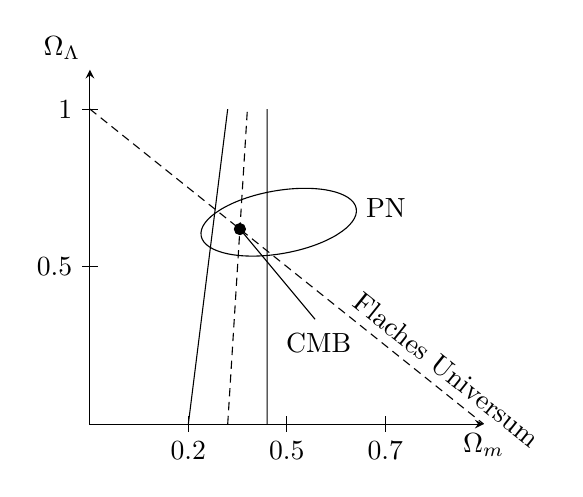
\begin{tikzpicture}[>=stealth]
				\draw[<->] (0,4.5)node[above left]{$\Omega_\Lambda$}--(0,0)--(5,0)node[below]{$\Omega_m$};
				\foreach \x \y in {0.5/2,1/4}{
					\draw (-0.1,\y)node[left]{$\num{\x}$}--++(0.2,0);
				}
				\foreach \x [count=\e] in {0.2,0.5,0.7}{
					\draw (\e*5/4,-0.1)node[below]{$\num{\x}$}--++(0,0.2);
				}
				\draw[densely dashed] (0,4)coordinate(a1)--(5,0)coordinate(a2)node[very near end,sloped,above]{Flaches Universum}(7/4,0)coordinate(a3)--(8/4,4)coordinate(a4);
				\draw (5/4,0)--(7/4,4)(9/4,4)--(9/4,0);
				\draw[fill=black] (intersection of a1--a2 and a3--a4)circle(2pt)coordinate(i);
				\draw[shorten <= 2pt, shorten >= 2pt] (i)--++(1,-1.2)node[below]{CMB};
				\draw[rotate=10] (i)++(0.5,0)ellipse(1cm and 0.4cm)++(1,0)node[right]{PN};
			\end{tikzpicture}
		\end{figure}
\end{itemize}
